\documentclass[12pt, a4paper]{report}

%% Dansk shizzle
\usepackage[utf8]{inputenc}
\usepackage[T1]{fontenc}
\usepackage[danish]{babel}

%% Sideopsætning
\usepackage{setspace}
\onehalfspacing
\usepackage{fix-cm}
\usepackage[a4paper,margin=2.5cm,headheight=2cm]{geometry}
\usepackage{lastpage}
\usepackage{fancyhdr}
\usepackage{graphicx}
\usepackage{sidecap}
\pagestyle{fancy} %skift til fancy
\fancyhead[L]{Kollegiekontoret}
\fancyhead[R]{\today}
\fancyfoot[L]{SUM2 Projekt}
\fancyfoot[C]{Side \thepage\ af \pageref{LastPage}}
\fancyfoot[R]{Team Awesome}


\setcounter{secnumdepth}{-1}
\title{SUM Projekt - Kollegiekontoret}
\author{Silas Fontain Jakobsen \and Tina Jensen \and Andreas Kristoffersen \and Jannie Gier Larsen \and Erik Holm Sejersen}
\date{21. Maj 2012}

% latex crash course: http://www.haptonstahl.org/latex/

\begin{document}
\begin{titlepage}
\maketitle
\end{titlepage}

\begin{abstract}
Forord
\end{abstract}

\tableofcontents

\chapter{Forundersøgelse}

\section{Forberedelse og projektgrundlag}
På vores indledende projektetableringsmøde blev vi enige om projektets omfang og blev enige om, at vi med al sandsynlighed ikke når at levere et færdigt og brugbart produkt indenfor den afsatte tid.

\subsubsection{Baggrund}
Vi har i forbindelse med en stillet eksamensopgave taget kontakt til Kollegiekontoret, da de har et kommende IT projekt med henblik på at få opgraderet deres hjemmeside til udlejning af ungdomsboliger.

\subsubsection{Opgaven og formål}
Vores opgaver består i at afdække Kollegiekontorets behov til en ny hjemmeside, der er tidssvarende og giver potentielle lejere et bedre overblik over deres muligheder for at leje en ungdomsbolig.

\subsubsection{Økonomiske og tekniske rammer}
Der er ikke afsat økonomiske midler til projektet, og vi kan ikke forvente der er mulighed for at tilføje flere ressourcer. Vores tekniske rammer og værktøjer er hvad vi har lært at anvende i studietiden, og der er hverken tid eller penge til større oplæring/kurser.

\subsubsection{Kritiske faktorer}
Det er ikke målet at vi på den afsatte tid når at udvikle et kørende system, og Kollegiekontoret forbereder sig også på at købe systemet af en anden leverandør. Vores mål med projektet er således dels at lære at anvende de lærte begreber og metoder, og dels at vise kollegiekontoret den agile side af udviklingsverdenen i praksis.

\subsection{Organisering}
\subsubsection{Projektets organisering}
Projektgruppen består primært at de fem undertegnede, hvoraf Tina Jensen er valgt som formel leder af gruppen. Kollegiekontorets interesser kan repræsenteres i projektgruppen af Silas F. Jakobsen der er medlem af Kollegiekontorets Forretningsudvalg. Kontakterne der arbejder til dagligt på Kollegiekontoret er informationsmedarbejder Lene Billeskov Jensen og administrationschef Diana Jørgensen. Andreas Kristoffersen er valgt som ansvarlig for versions- og dokumentstyring.
I princippet kunne en formel styregruppe etableres med kontaktpersonerne fra kollegiekontoret, men da dette også er et læringsprojekt vil vi alle gerne være lidt involveret i beslutningsprocesserne, og når hele projektgruppen indgår er det lidt strakt at kalde det en styregruppe.

\subsubsection{Ressourcer}
Uden tildelte økonomiske midler må vi anvende de gratis værktøjer vi kan få fat i, heldigvis er det er udbudet af gratis værktøjer ganske omfattende, og vi har opsat infrastruktur i form af dokumentstyring og versionskontrol, og vi har de nødvendige udviklingsværktøjer til rådighed.

\subsubsection{Interessenter}
Vi vurderer, at der på projektet findes følgende relevante og klart definerede interessenter:
\begin{itemize}
\item Kunde: Kollegiekontoret
\item Leverandør: Team Awesome
\item Projektleder: Tina Jensen
\item Slutbrugere: Nuværende og potentielle lejere af ungdomsboliger i Aarhus
\item Udviklere: Team Awesome
\item Testere: Team Awesome
\item Konsulent: Hanne Sommer
\end{itemize}

\begin{figure}[h!]
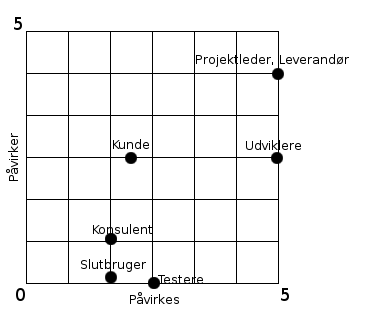
\includegraphics[width=0.5\textwidth]{interessenter}
\caption{Figur, der viser interessenternes indflydelse.}
\end{figure}

\begin{figure}[h!]
  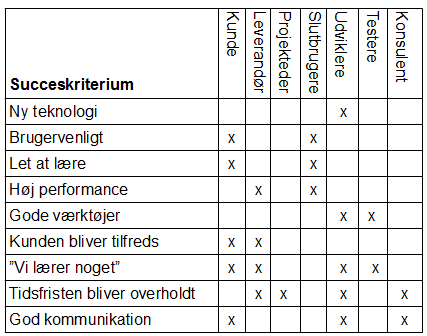
\includegraphics[width=0.5\textwidth]{succeskriterium}
  \caption{Figur, der viserinteressenternes succeskriterier .}
\end{figure}

En mulig konflikt i vores succeskriterier - i og med at der er tale om et skoleprojekt - kan være at vi som studerende har mere fokus på at lære noget, end at levere noget kunden kan bruge og bliver tilfreds med. Udviklingsforløbet er en læreproces for os, som derfor vil bruge længere tid på hver enkelt del end en udvikler fra erhvervslivet, og vi vil lave flere eksperimenter med hvordan produktet skal fungere, som måske ikke er forenlige med kundens forestillinger om et færdigt system.

Grundet projektets størrelse er det næppe sandsynligt at et færdigt system vil kunne leveres indenfor tidsfristen, er der opnået et fælles mål fra leverandørens såvel som fra kundens side, om fokus på læringsprocessen. For kunden er det vigtigt at opleve, hvordan et udviklingsforløb er. Det indebærer, at det i høj grad er leverandøren (og dermed også projektlederen), der i sidste ende tager beslutninger angående projektet.



\subsection{Risikoanalyse}
\subsubsection{Produkt}

\subsubsection{Proces}

\subsubsection{Personressourcer}
Hele holdet har taget en TRAP-test. Testen viste at holdet har balance i de fleste punkter men har en manglende evne i kommunikation. Holdet har ellers medlemmer, som har mindst 15 point i de andre kategorier mens den højeste scorer i kommunikation kun er ca. 11 point. Selvom kommunikationen er lav kender hele holdet hinanden forholdsvis godt, da vi har arbejdet sammen flere gange før.
TRAP-testen skal ikke ses som endegyldige fakta, men mere skal bruges som en test der giver et fingerpeg om hvordan gruppen er sammensat, og hvordan de enkeltes styrker dækker de andres svagheder ind. Testen giver også et overbliksbillede over gruppens generelle svagheder, som vi skal være særligt opmærksomme på. De områder hvor flere gruppemedlemmer er mindre stærke, kræver fælles indsats for at opnå bedst mulig synergi på området.

\begin{figure}[h!]
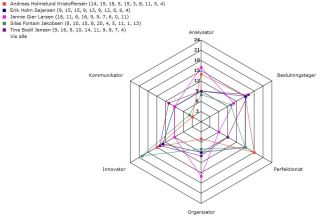
\includegraphics[width=0.5\textwidth]{itsaTRAP}
\caption{Figur, der viser resultatet af TRAP-testen.}
\end{figure}

\subsubsection{Aftaler og koordinering}
Møder med kollegiekontoret er umiddelbart aftalt i et fåtal, og vi forventer ikke at kunne bruge tid fast til at udvikle sammen med dem “ved siden af”. Møder aftales med Lene Billeskov Jensen.

\subsection{Metode}
\subsubsection{Overordnet fremgangsmåde}
Vi har lært om at bruge MUST-metoden, og det er overordnet denne metode vi vil anvende principper og værktøjer fra i forundersøgelsen. På vores plan kan ses overskrifter for de begreber vi har arbejdet med.

\subsubsection{Plan}
\begin{figure}[h!]
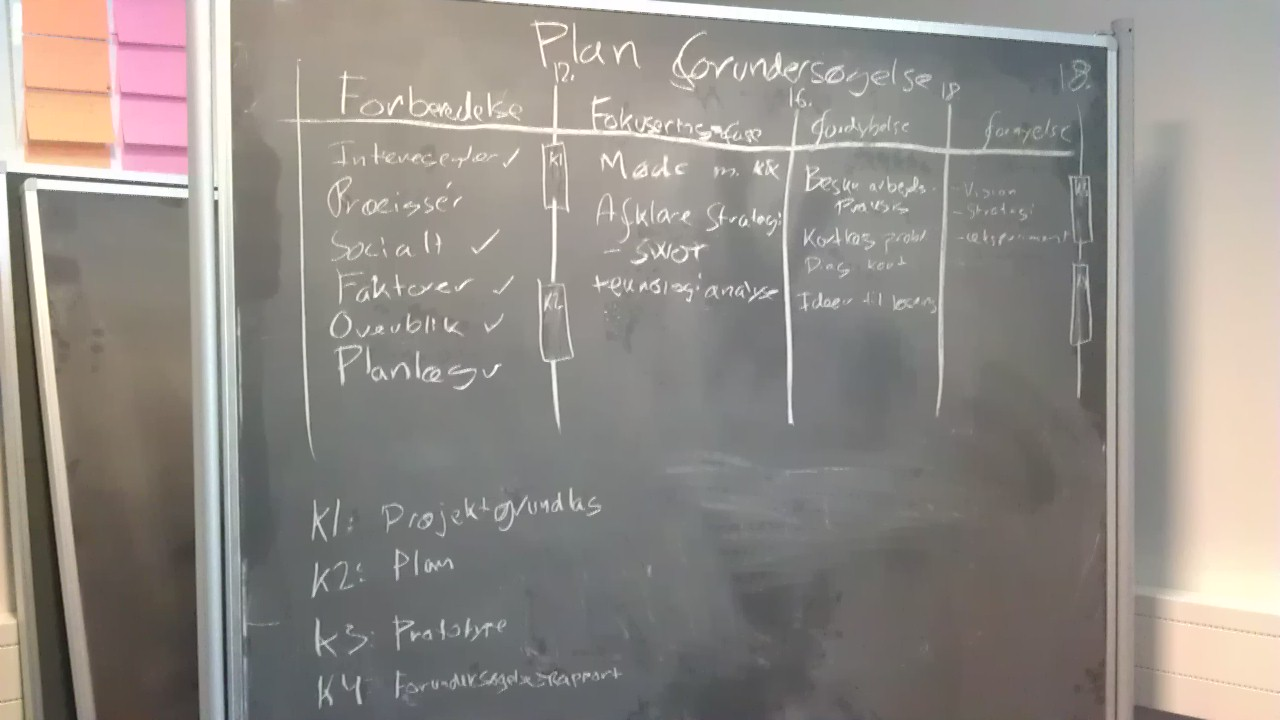
\includegraphics[width=0.5\textwidth]{forundersoegelsesplan.jpg}
\caption{Billede af planen.}
\end{figure}

\subsubsection{Teknikker og beskrivelsesværktøjer}
Til planen er allerede anvendt referencelinie-planlægning, og vi forventer at benytte os af interview/observation i forbindelse med at kortlægge arbejdspraksis (virksomhedsbesøg). Vi laver også en SWOT analyse, samt analyserer mål og strategi for at danne os et overblik og kortlægge problemstillingerne.

\subsubsection{Arbejdsform}
Internt i projektgruppen forventer vi at arbejde samme i løse grupper og individuelt i forbindelse med opgaveløsning. Samarbejdet med kollegiekontoret/styregruppe løftes med møder og email.
I det daglige vil vi bruge opslagstavler og alm. tavler til at holde styr på organiseringen.

\section{Fokusering}
\subsection{Virksomhedsbeskrivelse}
Hvis man er ung og skal i uddannelse eller er i gang med en uddannelse i Aarhus vil man med høj sandsynlighed benytte Ungdomsbolig Aarhus for at finde en bolig. På Ungdomsbolig Aarhus hjemmeside søger unge efter en ungdomsbolig. Hjemmesiden holder styr på unge der ansøger og boligforeninger som har boliger der skal beboes. De står for at udsende tilbud når boliger bliver frie, og for opsigelse af boliger.

  \subsubsection{Interne forhold}
De ansatte ved kollegiekontoret er primært kontorarbejdere der administrerer ungdomsboligerne igennem webbolig, der er et ERP værktøj for boliger. Arbejdet består bl.a i at tildele tilbud til ansøgere ved ledige boliger og opsige aftaler, samt rydde op i information som brugerne indtaster forkert, fx dobbelte ansøgninger. Opgaven er til dels papirtung da der anvendes udkørsler fra systemet som en oversigt over ledige boliger der skal tildeles. Arbejdsfordelingen er ret afklaret, og webbolig fungerer rimelig effektivt til at klare opgaven. Arbejdsgangen er tilrettelagt for at undgå fejl der kan medføre lejetab for de kollegier der administreres, omend i en idéel verden udføres der et arbejde der fra et teknisk synspunkt godt kunne automatiseres.

Ønsket om forandring ligger derimod i præsentationen af data ind/ud fra brugerne, der groft sagt er meget basal og uoverskuelig for mange. Der er ønsker om at gøre det lettere at udvælge relevante boliger i forbindelse med oprettelse af ansøgning, så det mindsker antallet af fejl brugerne laver, samt reducerer behovet for henvendelser fra ansøgere der ikke har kunnet overskue systemet.
  \subsubsection{Omgivelser}
Da man som ung boligsøgende under uddannelse reelt ikke har et andet alternativ end ungdomsbolig Århus har de tilnærmelsesvis opnået et markedsmonopol. Markedssituationen i sig selv må ses som værende stabilt, om end der typisk er større efterspørgsel end udbud. Det er dog ikke faktorer, som Kollegiekontoret som sådan hverken kan eller skal ændre på. Det er naturligvis nødvendigt at indrette sig efter den gældende lovgivning på området, og til dels også boligforeningerne, som de har et tæt samarbejde med.

\subsubsection{SWOT-analyse}
\begin{tabular}{ | l | r | }
\hline
Styrker & Svagheder \\ \hline
Markedsmonopol & Ingen konkurrence -> Ingen fornyelse \\
Stabilt marked & Umiddelbart ingen mulighed for markedsekspansion \\ \hline
Muligheder & Trusler \\
Teknologisk udvikling & \\
\hline
\end{tabular}
\newline
Idet Kollegiekontoret på dette område tilnærmelsesvis har monopol på markedet, har de ikke behov for at forny sig. De har dog heller ikke umiddelbart mulighed for det da markedets situation hele tiden er mere eller mindre stabil i forhold til målgruppen. De ønsker alligevel at levere en god service til deres brugere, hvor det ses at man kan udnytte den teknologiske udvikling til eks. at lave en bedre hjemmeside. Umiddelbart har de ingen eksterne trusler idet markedet er statisk.

  \subsubsection{IT-strategi}
Kollegiekontoret har ikke en decideret IT-strategi, men der er fokus på IT i deres aktivitetsmål. De relevante delmål går ud på at få bedre IT-systemer og lettere (kortere) arbejdsgange i administrationen. Disse mål skal opnås ved en mere sammenhængende elektronisk håndtering. Under mødet d. 16. april 2012 kom det også frem at de ønsker fremtidig fokus på brugervenlighed, som undgomsboligaarhus.dk skal afspejle. I den forbindelse har vi fået en behovspecifikation, som er baseret på feedback de har fået fra brugere.

  \subsection{Projektets arbejdsområder}
- Mere brugervenlig og tidssvarende brugeroplevelse af ungdomsboligaarhus.dk \newline
- Mere stabilt \newline
- Øget funktionalitet i præsentation af data og søgekriterier \newline

\section{Fordybelse}
\subsubsection{Referat af observationer og interviews}
\paragraph{Møde hos Kollegiekontoret d. 16/4-2012}
På mødet var der fokus på Kollegiekontorets bevæggrunde for ønske af et nyt system, og hvad de forventer det nye system skal kunne i forhold til det gamle. Der blev talt en del om at brugeren på den nye hjemmeside skal have en bedre oplevelse end på den gamle, samt at den nuværende hjemmeside har problemer med stabilitet, som den nye skal løse. Problemer med den nuværende arbejdssituation er udspecificerede i det diagnostiske kort nedenunder.
Desuden observerede vi, hvordan de bruger deres system i praksis og hvordan deres arbejdsproces med ansøgningerne og opdatering af hjemmesiden foregår. Dette havde til formål at finde frem til måder hvorpå det nye system kan effektivisere processen.

\subsubsection{Arbejdsgange}
\paragraph{Tildeling af bolig} foregår i webbolig, hvor en udlejningsmedarbejder har udkørsler med ledige boliger, der sammenholdes med en liste produceret i webbolig over ansøgere med længst anciennitet og evt. andre boligtilbud udsendt for nylig.

\paragraph{Retning af brugerdata} administreres ofte af medarbejderen, der må sidde med udkørsler og sammenligne brugere med enslydende navne for at rydde op i dobbelte ansøgere.

\subsection{Rige billeder}
Se Figur ~\ref{r_billede}
\begin{figure}
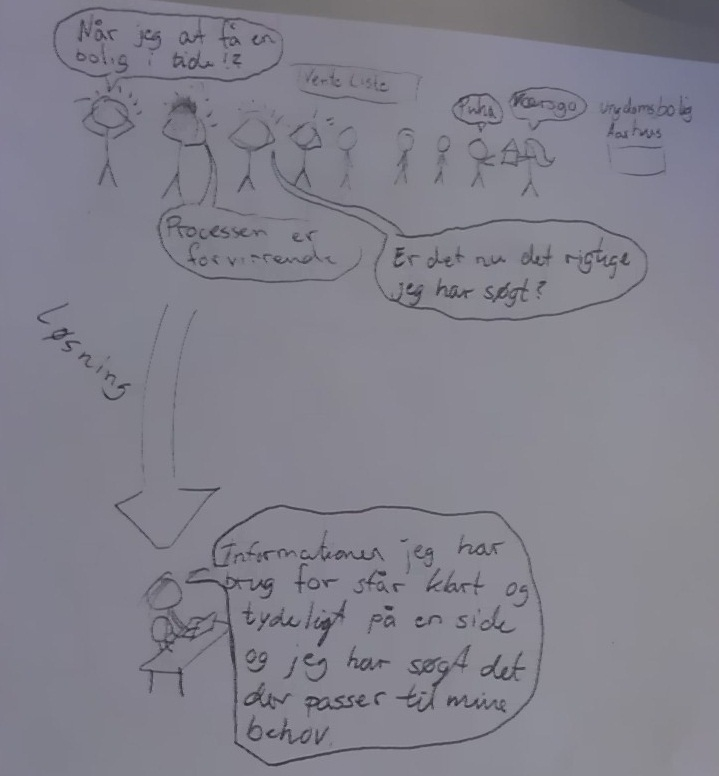
\includegraphics[width=0.5\textwidth]{rigtbillede}
\caption{Rigt billede.}
\label{r_billede}
\end{figure}

\subsection{Diagnostiske kort}
Se: Tabel ~\ref{d_kort}
\begin{table}
\caption{Diagnostiske kort}
\label{d_kort}
\begin{tabular}{| p{4cm} | p{4cm} | p{4cm} | p{4cm} |}
\hline
Problem & Årsag & Konsekvens & Ideer til løsning \\ \hline
Information forsvinder i systemet. \newline Siden kan kun bruges optimalt i IE. & Brugere logges ud under ansøgning. \newline Informationer kan forsvinde ved for mange opdateringer. \newline Bøvlet opdateringsproces. \newline Dårlig kode. & Frustrede ansøgere. \newline Klager. & Fejl lokaliseres. \newline Der startes forfra. \\ \hline

Siden er svær at navigere. & Layoutet er ikke intuitivt eller sammenhængende. & Brugeren finder ikke den ønskede information. & Mere gennemtænkt og brugervenligt layout. \\ \hline

Oprydning i information brugeren taster forkert. & Besværligt loginsystem & Ekstra arbejde med at vedligeholde data & Login systemet gentænkes \\ \hline

Bruger meget papir på store udkørsler. & Mange data der skal sammenholdes. & Papirspild & Bedre repræsentation af data i systemet \newline Opgraderet arbejdsplads med to skærme i stedet for én \\ \hline

Siden er uoverskuelig. & Mangel på søgekriterier. & Frustrerede ansøgere. \newline Ansøgere havner måske et sted de ikke havde tænkt sig. & Etablering af søgefunktion. \\ \hline

Besværlig login proces. & Autogenererede login oplysninger. & Ansøgerne opretter nye ansøgninger istedet for at bruge den allerede oprettede. & Brugerne får selv mulighed for at oprette et personligt login. \\ \hline

Nedbrud i systemer. & Forskellige leverandører af systemer til hjemmesider og webbolig. & Dyr vedligeholdelse og fejlretning. & Bedre kvalitet i løsninger. \newline Brug samme leverandør, giv dem et samlet ansvar. \\ \hline

\end{tabular}
\end{table}

\subsection{Mål}
\begin{enumerate}
\item Bedre browser kompatibilitet
\item Søgbare boliger med kriterier/valg
\item Nemt at ændre/vedligeholde informationer for personalet
\item Stabil hjemmeside
\item Brugervenligt layout
\item Individualiseret brugeroplevelse
\item Nemt login system
\item Integrering af geografisk placering i forhold til eks. uddannelsesinstitutioner
\item Integreres med webbolig
\end{enumerate}


\section{Fornyelse}
Samlet set er problemerne for Kollegiekontoret ikke så omfattende, og kræver ikke en større reorganisering af arbejdsgange, men hovedfornyelsen ligger hos kunderne som får en bedre service, lettere adgang til information og alt i alt en bedre oplevelse.

\subsection{Visioner om den samlede forandring}
\subsubsection{Vision 1}
Tilretning af eksisterende hjemmeside, hvor den oprindelige kode opgraderes med yderligere funktionalitet og nuværende fejl rettes så brugerne får en bedre oplevelse med hjemmesiden og der bliver færre inputfejl at rette i de bagvedliggende data.

Dennes vision er ikke let at implementere i praksis, da vi ikke har adgang til det eksisterende system internt, og da det er så ukompatibelt med de nye tanker om hvordan systemet skal virke at det ville være urentabelt at bruge denne fremgangsmåde. Fordelen kunne være at det ville være en billig lappeløsning på problemerne, men de eksisterende småproblemer kan vokse sig større. Det kunne også være at systemet er konstrueret dårligt og derfor ville tage lang tid at sætte sig ind i systemet og rette på det uden at forårsage nye fejl.

\subsubsection{Vision 2}
Gentænkning af systemet og efterfølgende ny implementation, hvor der skrives helt ny kode helt fra bunden af, og alle eksisterende fejl derfor elimineres og ny funktionalitet kan tilføjes uden hensyntagen til kompatibilitet med oprindelige systemer.

Dette kan gennemføres i praksis og være en rentabel løsning. Det tager sandsynligvis ikke længere tid end at rette i den eksisterende løsning, og resultatet vil være mere helt, og lettere og billigere at opdatere i fremtiden, og det vil være lettere at udføre vision 3.

\subsubsection{Vision 3}
Implementation af integrering af Webbolig, som er en udbygning af scenariet beskrevet i Vision 2, og indebærer fuld kompatibilitet med systemet Webbolig.

En fuld integration vil være meget svær at kunne lave på den afsatte tid. Det er derfor ikke noget vi vil bestræbe os på at opnå, men det er et oplagt fremtidsprojekt.

\subsection{Strategi og plan for realisering}
Taget i betragtning af den stramme tidsplan og manglende kendskab til eksisterende løsning, er vision 2 en realistisk løsning for skoleopgaven, men vision (2+)3 er den endelige løsning for Kollegiekontoret. Det eksisterende system er en meget forældet platform der kan blive meget dyr at vedligeholde i fremtiden efterhånden som færre udviklere har kendskab til systemet.

\subsection{Mock-ups}
Se bilag

\section{Konklusion på forundersøgelse}
Vi har været godt rundt om Kollegiekontoret, og afklaret at de har et reelt behov for en tidsvarende hjemmeside der giver en bedre servicering af ansøgere. Der er lagt op til at projektgruppen, som omfatter os som studerende implementerer vision 2 bl.a. pga. den begrænsede tid. Den manglende integrering med webbolig får ikke konsekvenser for Kollegiekontoret da de ikke regner med at få et kørende system.


\chapter{Bilag}

\begin{SCfigure}
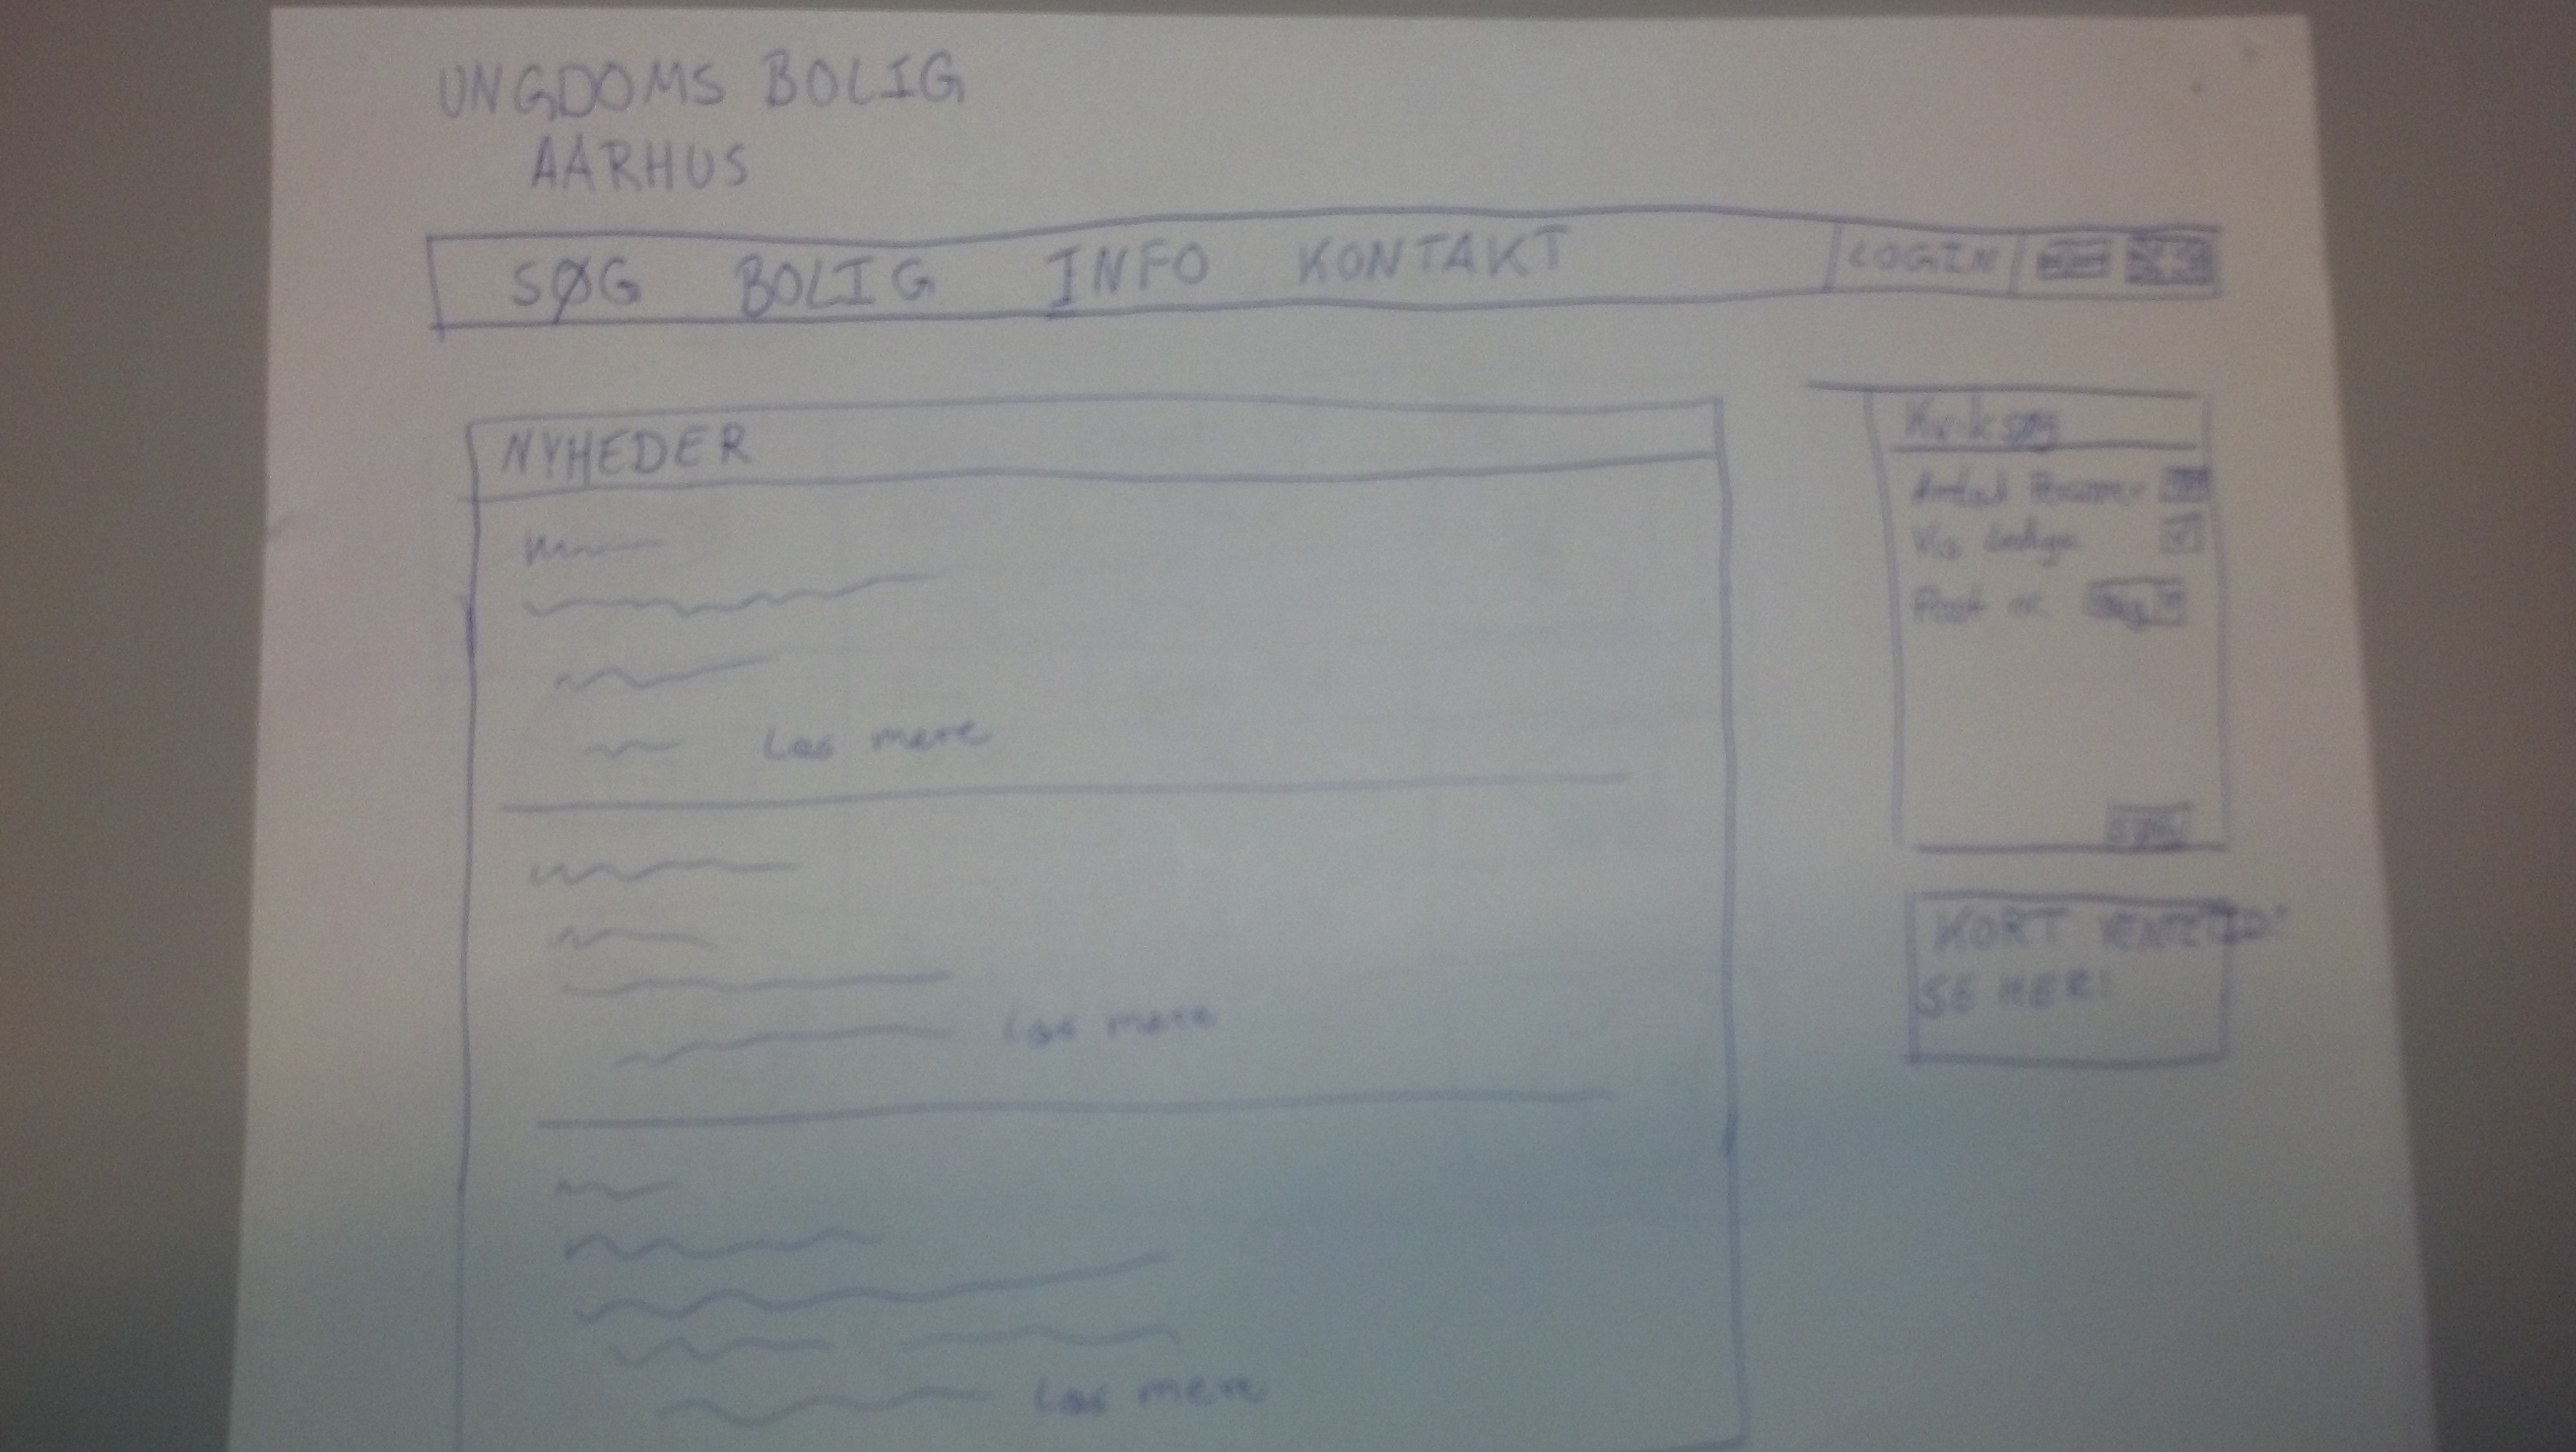
\includegraphics[width=0.5\textwidth]{eksperiment_forside}
\caption{Eksperiment: Forside med nyheder som hovedelementet, en simpel menu i toppen giver bedre overblik og navigation}
\label{e_forside}
\end{SCfigure}

\begin{SCfigure}
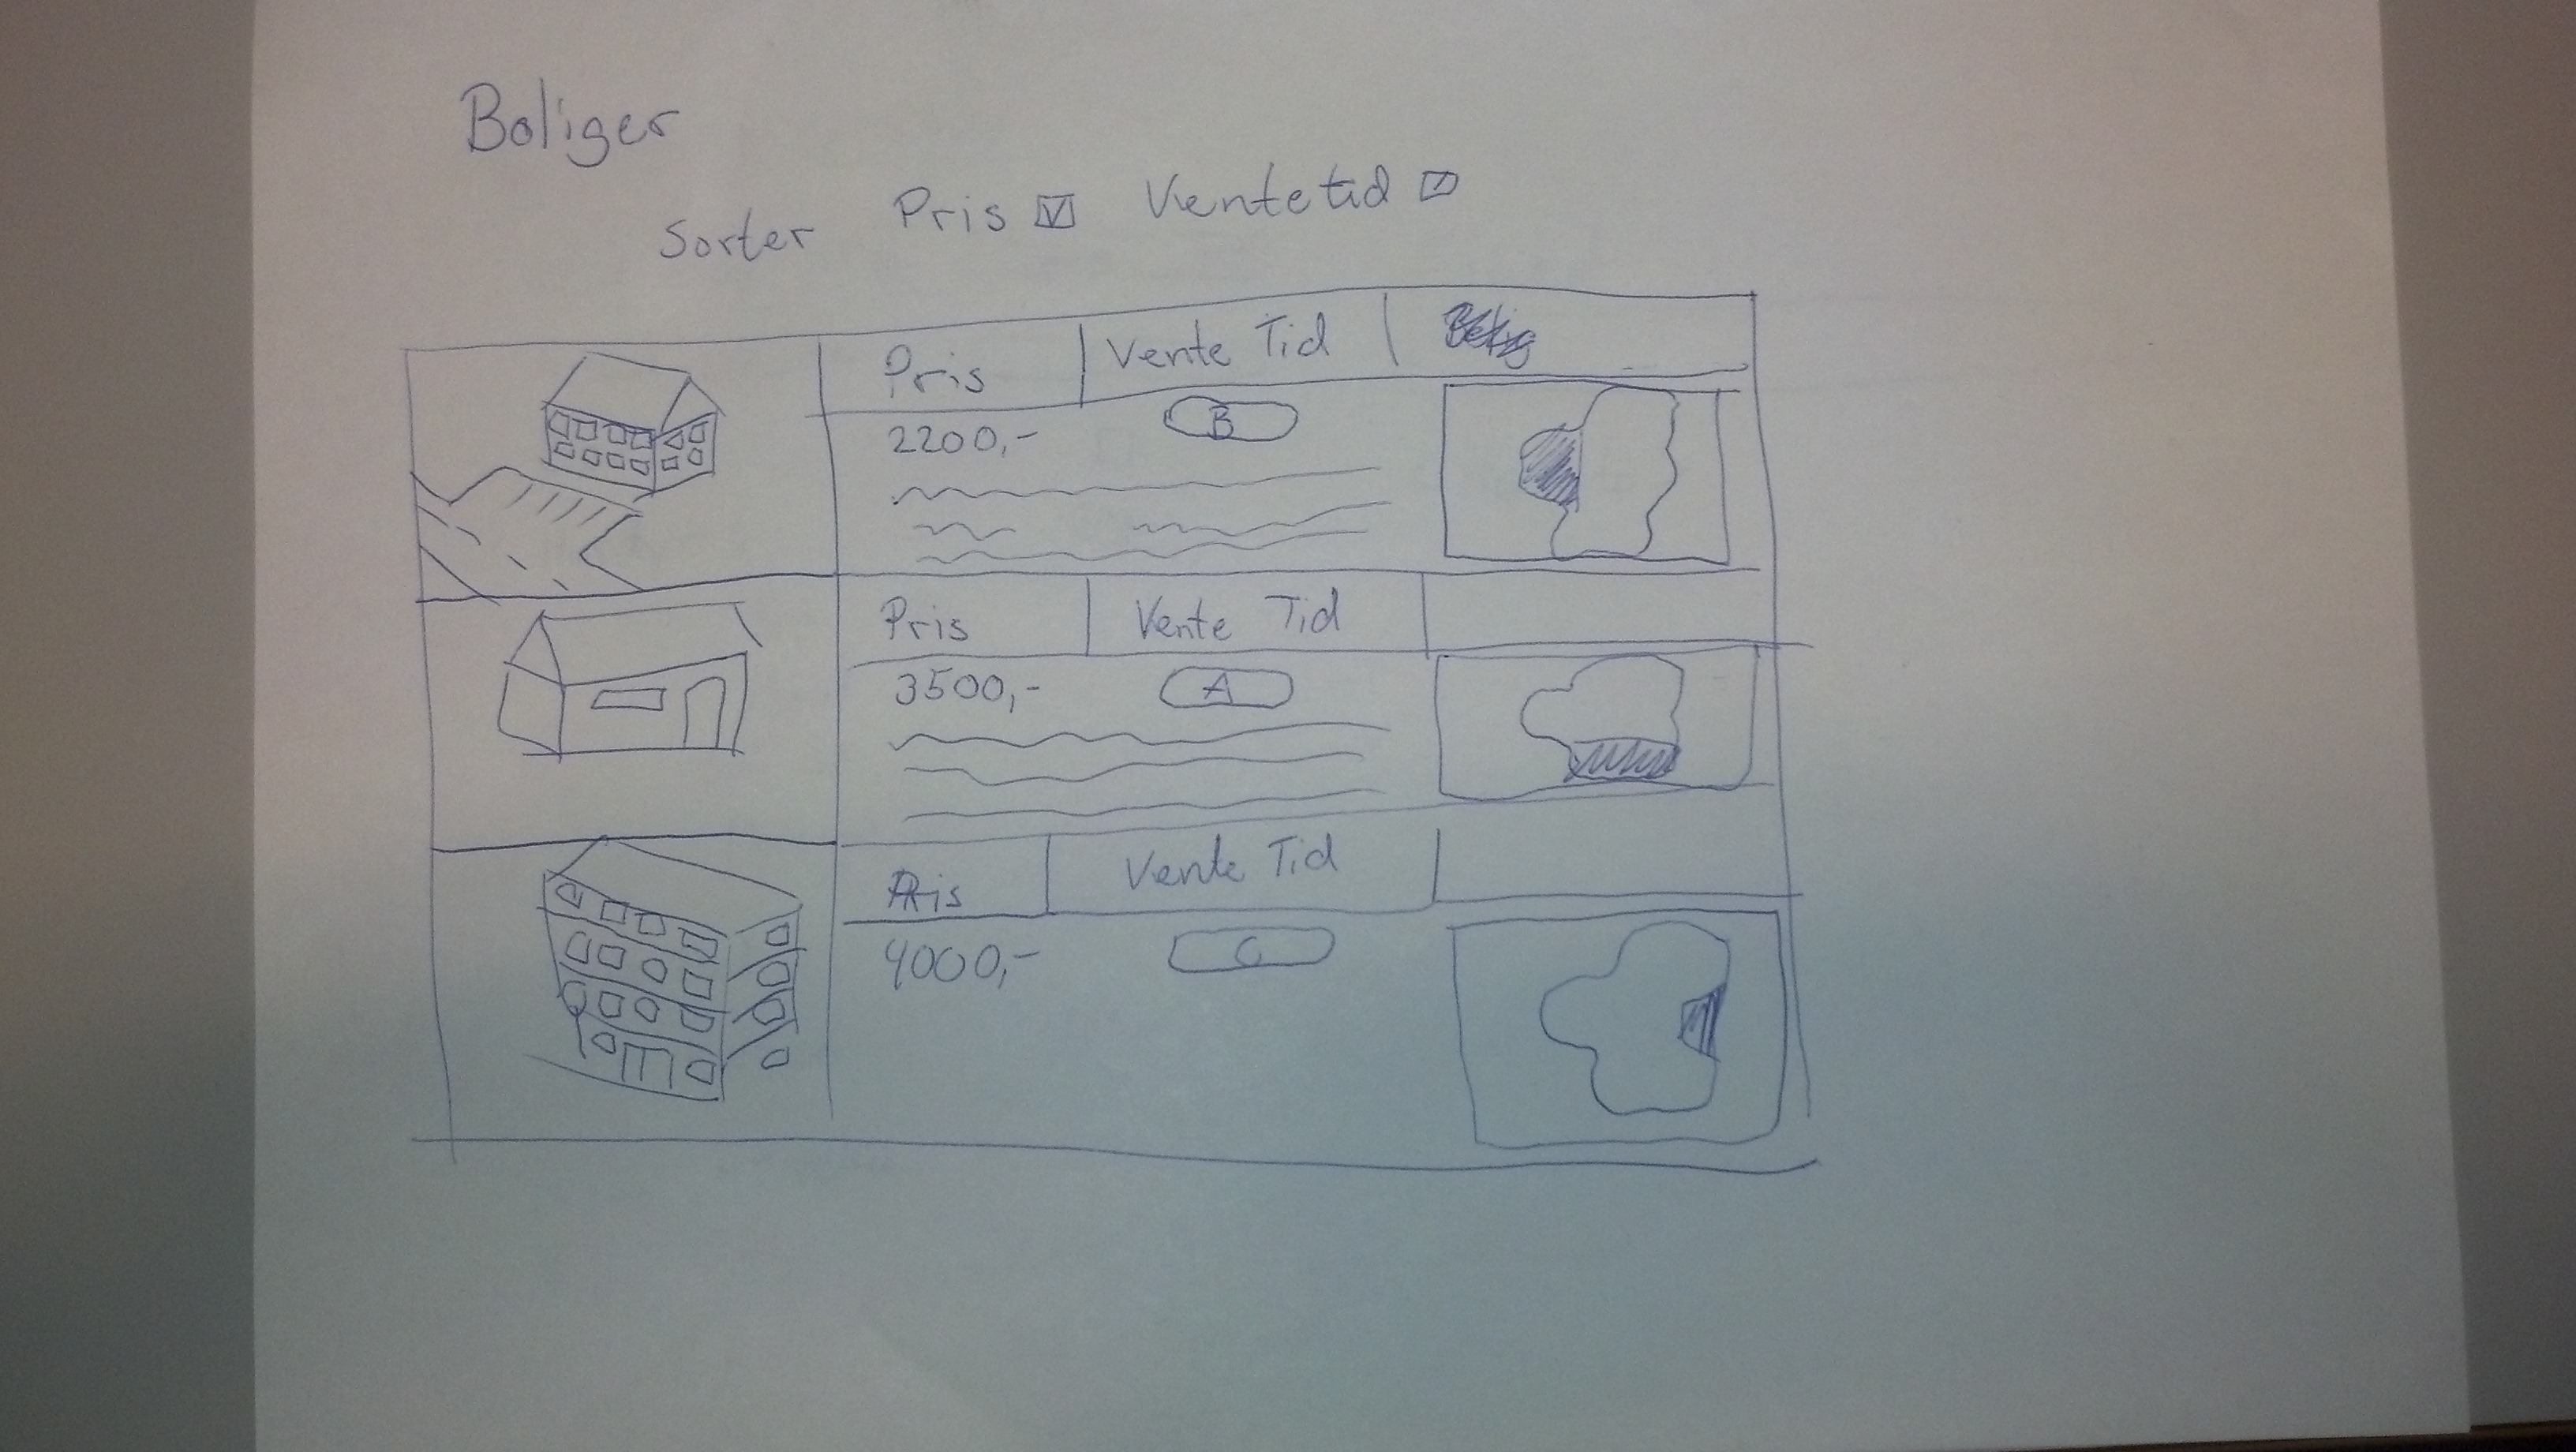
\includegraphics[width=0.5\textwidth]{eksperiment_liste}
\caption{Eksperiment: Liste / Søgeresultat med fokus på det værelse der passer til søgningen men stadig med data fra den afdeling det hører under}
\label{e_liste}
\end{SCfigure}

\begin{SCfigure}
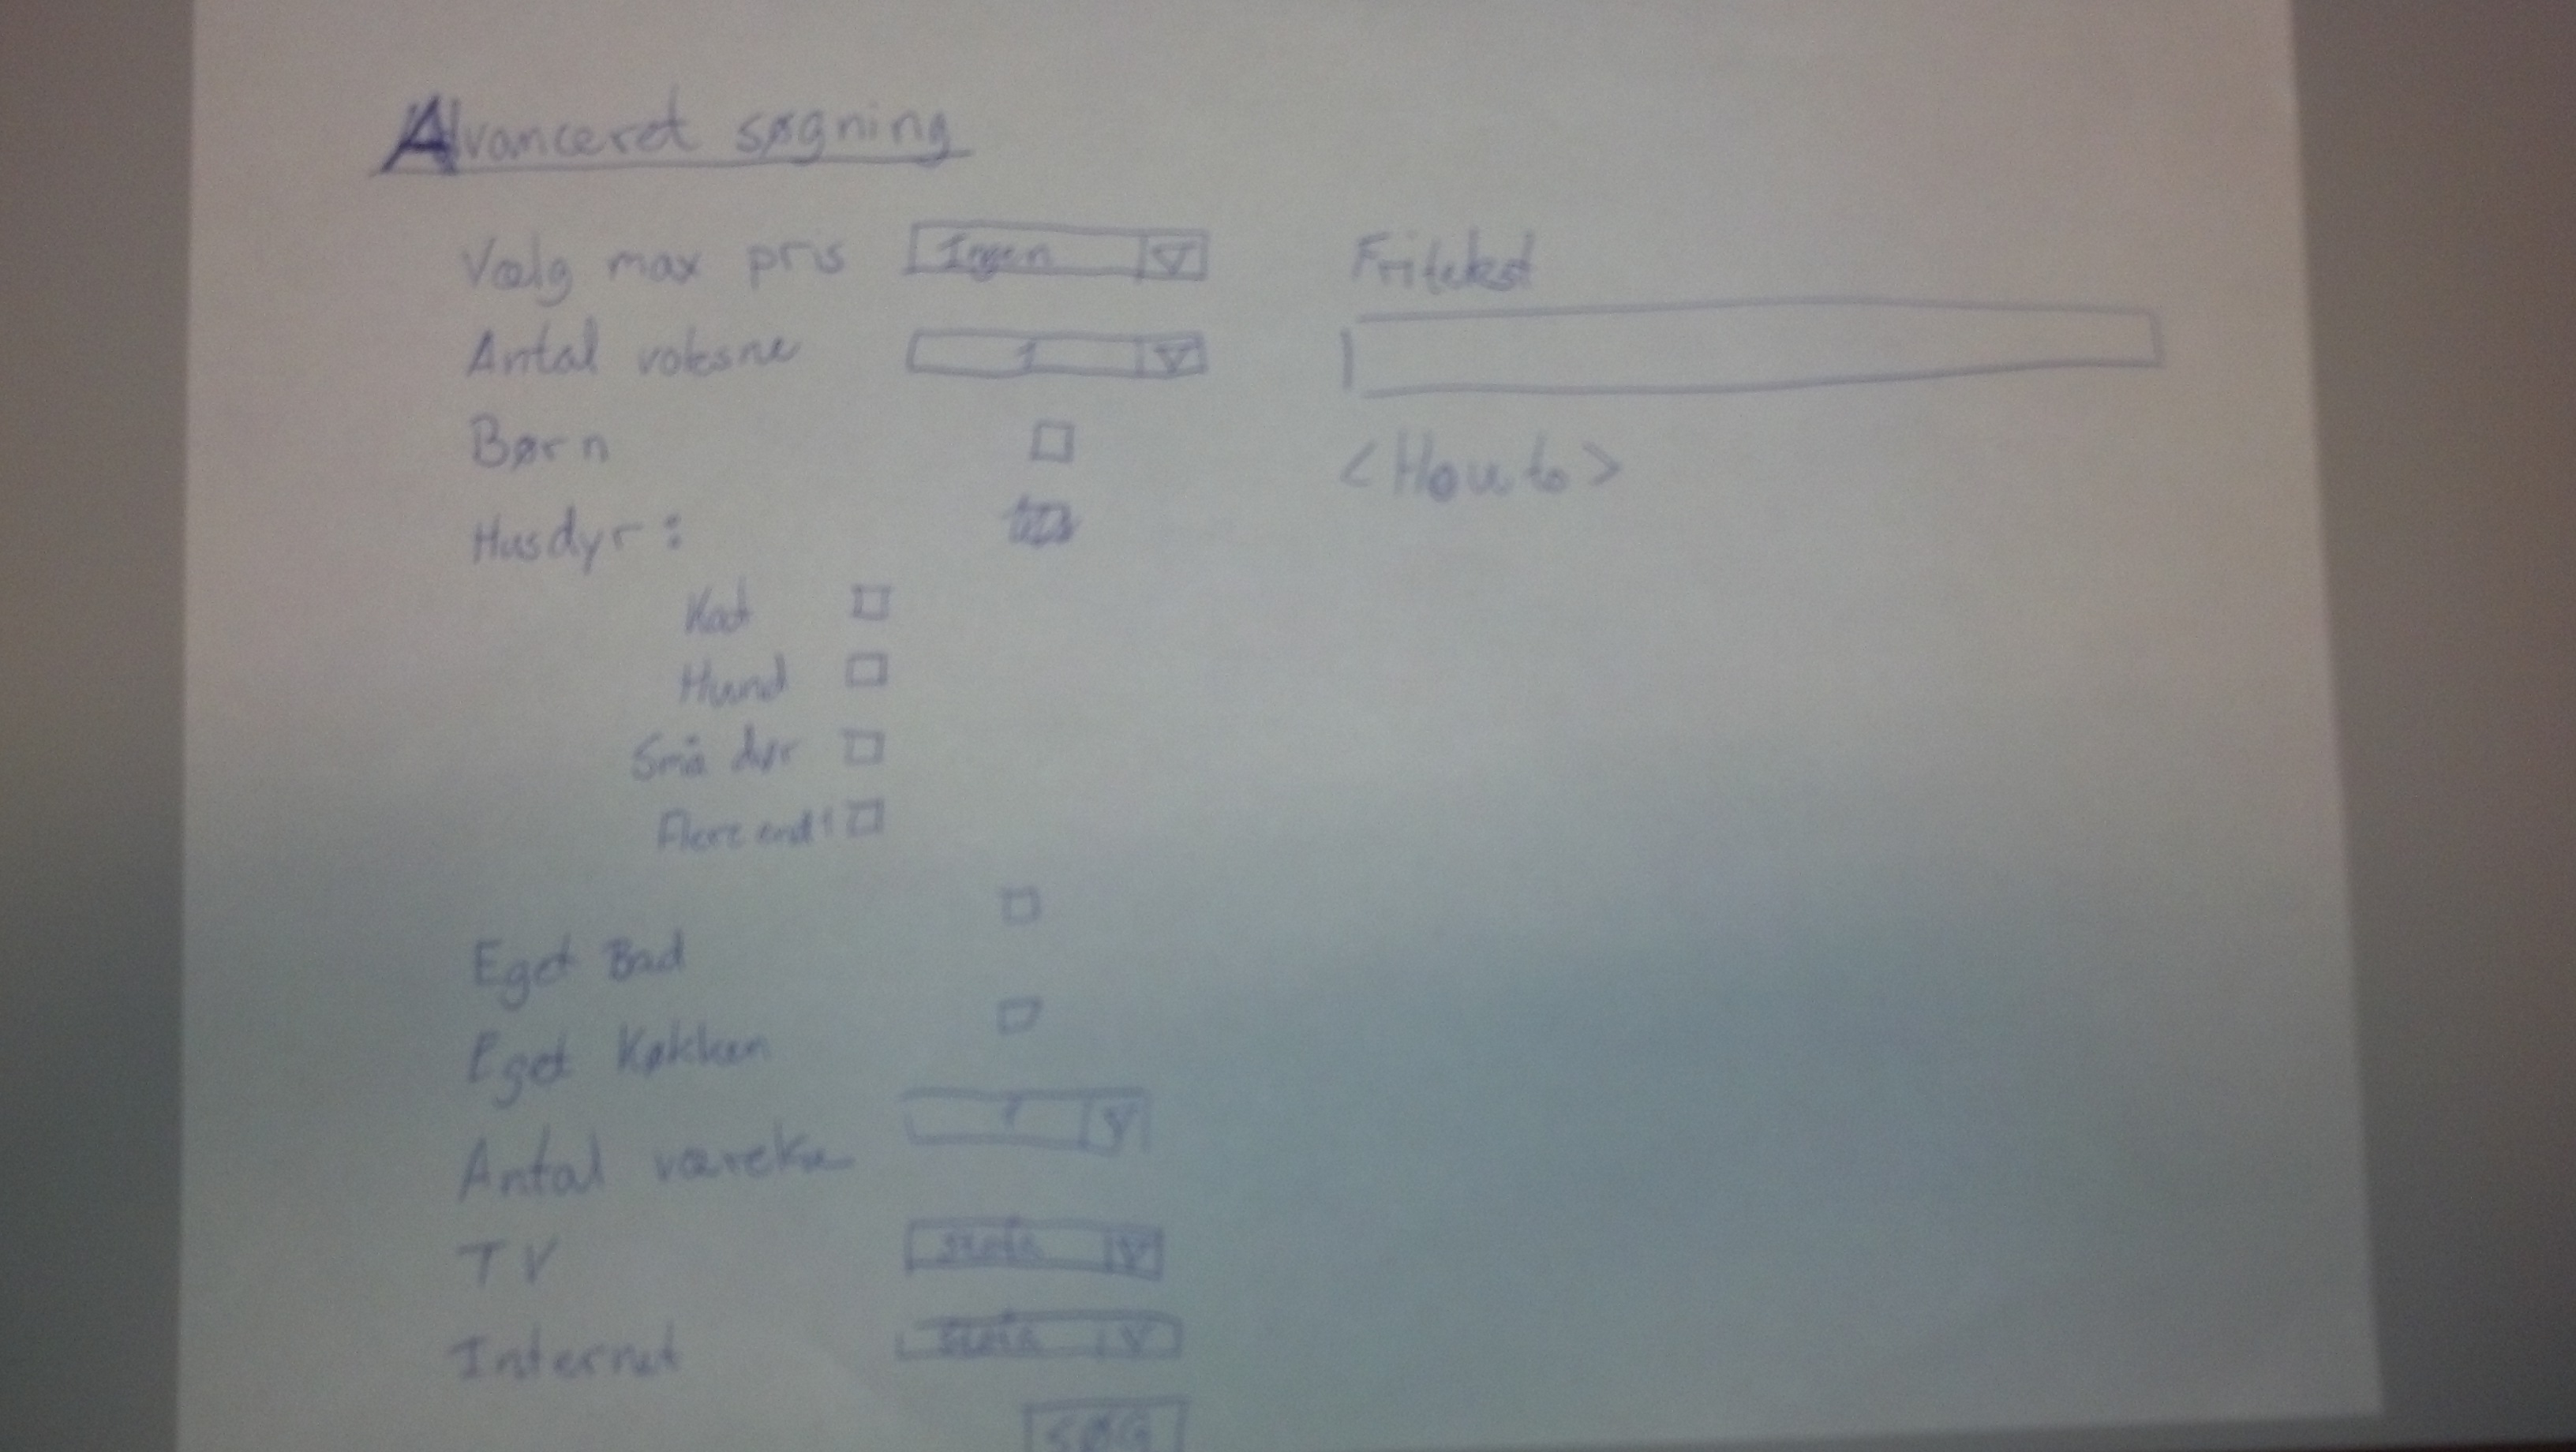
\includegraphics[width=0.5\textwidth]{eksperiment_soeg}
\caption{Eksperiment: Avanceret søgning. Overblik over de muligheder der kunne være i en avanceret og tilpasset søgning, layout vil blive optimeret.}
\label{e_soeg}
\end{SCfigure}

\end{document}

